\graphicspath{ {./images/11_Data_export} }
\newpage

\section{Data export}
In the \menu{Data export} tab you can download the processed data as in \texttt{.xlsx} format or as an R object. 

The processed data includes:

\begin{itemize}[topsep=0pt, itemsep=0pt]
	\item Sample names, sample types and sample IDs.
	\item Plate wells (if applicable).
	\item Uploaded metadata (if applicable).
	\item Sum intensities of all glycosylation sites.
	\item Relative abundances of all analytes.
	\item Calculated glycosylation traits, protein quantities and/or site occupancies (if applicable).
\end{itemize}

Additionally, you can download a data processing report in HTML format, which can be opened in any browser.
This report contains the GlycoDash version that was used, the names of uploaded files, choices that were made during each processing step, and all data visualizations.
The generated plots retain their interactivity in the HTML report.

There is also a section where you can make notes (e.g, about why you made certain choices during spectra or analyte curation).
These notes will be added to the bottom of the HTML report.

\begin{center}
	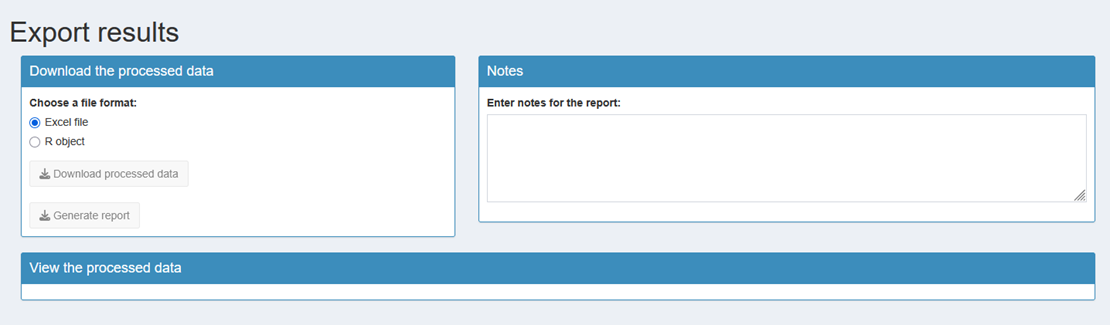
\includegraphics[scale=0.5]{export.png}
\end{center}